% packages
\PassOptionsToPackage{dvipsnames}{xcolor}  % needed to get colors working in certain environments
\documentclass[titlepage,11pt,a4paper,ngerman]{article}
\usepackage[utf8]{inputenc}
\usepackage[T1]{fontenc}
\usepackage[german]{babel}
\usepackage{graphicx}
\usepackage{wrapfig}  % used for wrapping a figure alternative to using minipages
\usepackage{amsmath}
\usepackage{amsfonts}
\usepackage{amssymb}
\usepackage[hidelinks]{hyperref}  % removes coloring for links
\usepackage{cleveref}
\usepackage{tikz}
\usepackage{tikz-cd}
\usepackage{nicefrac}  % adds \nicefrac alternative to regular \frac
\usepackage{mathtools}
\usepackage{enumerate}
\usepackage{cancel}  % adds \cancel which adds strikethrough
\usepackage{tocloft}
\usepackage{tcolorbox}
\usepackage{bm}  % adds \bm to make symbols bold, replaces outdated \boldsymbol
\usepackage[shortlabels]{enumitem}
\usepackage{placeins}
\usepackage{booktabs}
\usepackage{wasysym}

\usepackage[margin=1in]{geometry}  % changes the margins on all pages
\usepackage{url}

%SI-unix
%\usepackage{array}
\usepackage[per=slash,
            decimalsymbol=comma,
			loctolang={DE:ngerman,UK:english},
			]{siunitx}	
\sisetup{locale = DE}

\usetikzlibrary{calc}
\usetikzlibrary{decorations.pathmorphing,patterns}
\usetikzlibrary{arrows}
\usetikzlibrary{decorations.pathreplacing}
%\usetikzlibrary{snakes}

% Andrez:
%\usepackage{epigraph}  % adds \epigraph used to add fancy quotes to the beginning of chapters
%\usepackage{fancyhdr}
%\setlength{\parskip}{1em}
%\setlength{\headheight}{35pt}
%\setlength\epigraphwidth{.8\textwidth}
% alt math font
%\usepackage{eulervm}  % switches to alternate math font, usually requires extra download


%Environments und Newcommands:


% general commands

% zu zeigen symbol
\newcommand{\zz}{\fontfamily{cmss} \selectfont{Z\kern-.61em\raise-0.7ex\hbox{Z}:}}
% build over
\newcommand{\bov}[2]{\buildrel{#2} \over{#1}}
% better looking := (defined as)
\newcommand*{\defeq}{\mathrel{\vcenter{\baselineskip0.5ex \lineskiplimit0pt \hbox{\scriptsize.}\hbox{\scriptsize.}}}=}
\newcommand*{\eqdef}{=\mathrel{\vcenter{\baselineskip0.5ex \lineskiplimit0pt \hbox{\scriptsize.}\hbox{\scriptsize.}}}}

% integral differential d
\newcommand{\dif}{\mathop{}\!\mathrm{d}}
\newcommand{\difi}[1]{\mathrm{d}#1\mathop{}\!}

\newcommand{\prt}[2]{\frac{\partial #1}{\partial #2}}  % used for partial derivatives, tip: input #1 can be left blank
\newcommand{\prd}[2]{\frac{\tx{d} #1}{\tx{d} #2}}  % used for absolute (standart) derivatives, tip: input #1 can be left blank

\newcommand{\dd}{\tx{d}}


%Mathe:
\newcommand{\verteq}{\rotatebox{90}{$\,=$}}  % used for commands below
\newcommand{\equalto}[2]{\underset{\scriptstyle\overset{\mkern4mu\verteq}{#2}}{#1}}  % adds equal to underneath
\newcommand{\equaltoup}[2]{\overset{\scriptstyle\underset{\mkern4mu\verteq}{#2}}{#1}}  % adds equal to above
\newcommand{\custo}[3]{\underset{\scriptstyle\overset{\mkern4mu\rotatebox{-90}{$\,#1$}}{#3}}{#2}}  % same as above but replaces equal sign with input #1
\newcommand{\custoup}[3]{\overset{\scriptstyle\underset{\mkern4mu\rotatebox{-90}{$\hspace{-3pt} #1$}}{#3}}{#2}}
\newcommand{\casess}[4]{\left\{ \begin{array}{ll} {#1} & {#2} \\ {#3} & {#4} \end{array} \right.}  % used to indicate to the reader that something is missing here


%Text:
\newcommand{\tx}[1]{\textrm{#1}}
\newcommand{\const}{\tx{const.}}

\newcommand{\ul}[1]{\underline{#1}}
\newcommand{\ol}[1]{\overline{#1}}
\newcommand{\ub}[1]{\underbrace{#1}}
\newcommand{\ob}[1]{\overbrace{#1}}

\newcommand{\hfw}{\color{RubineRed}\tx{ $\star$hier fehlt was$\star$ } \color{black}}  % used to indicate to the reader that something is missing here 


%Spezielles:


%Theo:
\newcommand{\lag}{\mathcal{L}}  % used for Lagrange function
\newcommand{\ham}{\mathcal{H}}  % used for Hamiltonian function
\newcommand{\gre}{\mathcal{G}}  % used for Green's function
\newcommand{\eofr}{\vec{E}(\vec{r})}
\newcommand{\pofr}{\Phi(\vec{r})}
\newcommand{\grr}{\mathcal G(\vec{r},\vec{r}')}
\newcommand{\vphi}{\varphi}
\newcommand{\vabla}{\vec{\nabla}}


%LA:
\newenvironment{bew}[1]{\subsection{Bew: #1}}{\hfill$\square$}
\newcommand{\Bew}[2]{\begin{bew}{#1}#2\end{bew}}
\newcommand{\enph}{F: V \to V \textrm{ Endomorphismus}}

\newcommand{\im}{\tx{im}}
\newcommand{\spa}{\tx{span}}
\newcommand{\adj}{\tx{adj}}
\newcommand{\grad}{\tx{grad}}
\newcommand{\ord}{\tx{ord}}

\newcommand{\basis}[3]{\{#1_{#2}, \dots, #1_{#3}\}}
\newcommand{\ska}[2]{\langle #1 , #2 \rangle}  % scalar product of input 1, and 2 can also be used for braket notation
\newcommand{\dmat}[3]{\begin{pmatrix} #1_{#2}&&\\ &\ddots& \\ && #1_{#3} \end{pmatrix}}


%Ex:
\newcommand{\kq}{\frac{1}{4\pi\epsilon_0}}  % writes out the whole constant k from electrostatic
\newcommand{\kqq}{\frac{\mu_0}{4\pi}}  % writes out the constant from magnetostatic
\newcommand{\uind}{U_{\tx{ind}}}
\newcommand{\folie}[1]{\color{gray}[Folie: #1]\color{black}}  % used to tell the reader that there was multimedia content during a lecture
\newcommand{\versuch}[1]{\color{red!50!black} \textbf{Versuch:} \color{black} \textbf{#1}\\ }  % used to tell the reader that there was a live experiment

\newcommand{\mau}{$\buildrel \mathcal{O} \over{\textbf{.}}$}  % the extreme Waldmann exclamation mark recreated in latex by Markus


% Lab commands:
\newcommand\mean{\begin{equation}
\frac{\sum_{i=1}^n x_i}{n}\label{mean}
\end{equation}}  % shortcut for the standard Mean function

\newcommand\meanstd{\begin{equation}
s_x=\sqrt{\frac{1}{n-1}\sum_{i=1}^n(x_i-\overline{x})^2}\label{meanstd}
\end{equation}}  % shortcut for the standard derivative mean function

\newcommand\prodquo{\begin{equation}\left\vert\frac{\Delta z}{z}\right\vert=\sqrt{\left(a\frac{\Delta x}{x}\right)^2+\left(b\frac{\Delta y}{y}\right)^2+\ldots}\textrm{ f\"ur }z=x^a\ y^b\ldots\end{equation}}

\newcommand\tfuncd{\begin{equation}
t=\frac{\vert x_n-y_n\vert}{\sqrt{x_s^2+y_s^2}}
\end{equation}}

\newcommand\tfunc{\begin{equation}
t=\frac{\vert x-y_0\vert}{u_x}
\end{equation}}


% ANDREZ
%\newcommand{\summ}[2]{\sum_{#1}^{#2}}
%\newcommand{\intt}[2]{\int_{#1}^{#2}}
\newcommand{\lcom}[1]{\color{MidnightBlue}#1\color{black}}  % used to indicate to the reader that this content was transcribed from the lecture
\newcommand{\bei}{\emph{Beispiel:}}
\newcommand{\bem}{\emph{Bemerkung:}}


% Boxen:

\tcbuselibrary{theorems}

% mahlt eine box nur um den text mit titel
\newtcbox{\fribox}[1]{nobeforeafter,colback=white,colframe=red!75!black,fonttitle=\bfseries,title=#1,sharp corners,tcbox raise base}

% mahlt eine große box um alles mit titel
\newcommand{\frbox}[2]{\begin{tcolorbox}[colback=white,colframe=red!75!black,fonttitle=\bfseries,title=#1]#2\end{tcolorbox}}

% mahlt eine box nur um den text
\newtcbox{\ribox}{nobeforeafter,colback=white,colframe=red!75!black,sharp corners,tcbox raise base}

% mahlt eine große box um alles was drinnen ist
\newcommand{\rbox}[1]{\begin{tcolorbox}[colback=white,colframe=red!75!black]#1\end{tcolorbox}}

% mahlt eine box um mathe innerhalb mathmode
\newcommand{\rmbox}[1]{\tcboxmath[colback=white,colframe=red!75!black]{#1}}

% super box (looks like regular boxed but wraps around anything)
\newenvironment{supbox}{\begin{tcolorbox}[colback=white,colframe=black,sharp corners,boxrule=.5pt]}{\end{tcolorbox}}

% the Big Black Box, can be used to separate examples or review material from the main text (used for Wiederholung)
\newcommand{\bbb}[2]{\begin{tcolorbox}[colback=white,colframe=black,fonttitle=\bfseries,title=#1,sharp corners,tcbox raise base]#2\end{tcolorbox}}

% array type box with title
\newenvironment{zebox}[1]{\begin{array}{|c|}
		\multicolumn{1}{l}{\tx{#1}} \\
		\hline
		\displaystyle
	}{\\ \hline
\end{array}}

% arrow list
\newlist{arrowlist}{itemize}{1}
\setlist[arrowlist]{label=$\Rightarrow$}


% optional:

\renewcommand{\vec}[1]{\bm{#1}}

% changed because of preferred looks
\renewcommand{\epsilon}{\varepsilon}
\renewcommand{\paragraph}[1]{\subsubsection{#1}}  % changed oddly behaving paragraphs to simple subsubsections which are not numbered nor in the toc

% nur in Theo benutzt !!!
% \renewcommand{\Phi}{\varPhi}

% evtl:
% \renewcommand{\boxed}{\rmbox}


% Tikz definitions:

\def\centerarc[#1](#2)(#3:#4:#5)% Syntax: [draw options] (center) (initial angle:final angle:radius)
{ \draw[#1] ($(#2)+({#5*cos(#3)},{#5*sin(#3)})$) arc (#3:#4:#5); }

\def\checkmark{\tikz\fill[scale=0.4](0,.35) -- (.25,0) -- (1,.7) -- (.25,.15) -- cycle;}  % checkmark used for proofs

\tikzset{
	annotated cuboid/.pic={
		\tikzset{%
			every edge quotes/.append style={midway, auto},
			/cuboid/.cd,
			#1
		}
		\draw [every edge/.append style={pic actions, densely dashed, opacity=.5}, pic actions]
		(0,0,0) coordinate (o) -- ++(-\cubescale*\cubex,0,0) coordinate (a) -- ++(0,-\cubescale*\cubey,0) coordinate (b) edge coordinate [pos=1] (g) ++(0,0,-\cubescale*\cubez)  -- ++(\cubescale*\cubex,0,0) coordinate (c) -- cycle
		(o) -- ++(0,0,-\cubescale*\cubez) coordinate (d) -- ++(0,-\cubescale*\cubey,0) coordinate (e) edge (g) -- (c) -- cycle
		(o) -- (a) -- ++(0,0,-\cubescale*\cubez) coordinate (f) edge (g) -- (d) -- cycle;
		\path [every edge/.append style={pic actions, |-|}]
		%(b) +(0,-5pt) coordinate (b1) edge ["\cubex \cubeunits"'] (b1 -| c)
		%(b) +(-5pt,0) coordinate (b2) edge ["\cubey \cubeunits"] (b2 |- a)
		%(c) +(3.5pt,-3.5pt) coordinate (c2) edge ["\cubez \cubeunits"'] ([xshift=3.5pt,yshift=-3.5pt]e)
		;
	},
	/cuboid/.search also={/tikz},
	/cuboid/.cd,
	width/.store in=\cubex,
	height/.store in=\cubey,
	depth/.store in=\cubez,
	units/.store in=\cubeunits,
	scale/.store in=\cubescale,
	width=10,
	height=10,
	depth=10,
	units=cm,
	scale=.1,
}


% other settings
\hbadness=99999  % removes unnecessary hbadness warnings

% the following are used to circumvent Roman numerals in the toc from running out of space
%\addtolength{\cftchapnumwidth}{10pt}
%\addtolength{\cftsecnumwidth}{10pt}
%\addtolength{\cftsubsecnumwidth}{10pt}
%\renewcommand{\thechapter}{\Roman{chapter}}  % just don't do this :)

% coloring
% for working at night
%\pagecolor{darkgray}
%\color{white}

\begin{document}

\title{
	\large Physiklabor für Anfänger*innen 2 \\
	Ferienpraktikum im Wintersemester 2019 \\[4mm]
	\textbf{\LARGE 
		Versuch Projektpraktikum:\\[3mm]
		Vermessung der Strahlungscharakteristik einer Dipolantenne
			} \\[3mm]
	(durchgeführt am 8. April bis 12. April 2019 bei Assistent: Dennis Sperlich) \\}
\author{Erik Bode, Damian Lanzenstiel, Markus Österle, Jan-Philipp Maurer \\ (Gruppen 111 und 22)}
\date{\today}
\maketitle
\tableofcontents
%\listoffigures
%\listoftables

% Document

\section{Veruschsziel}

Das Ziel des Versuches ist es, eine Dipol-Antennen zu bauen und diese zu nutzen um ihre Strahlungscharakteristik zu bestimmen. Wenn noch Zeit übrig wäre, sollte das HackRF und eine Drohne genutzt werden um Antennen in der Gegend zu vermessen.

\section{Labortagebuch}

\subsection{Tag 1}

Zu Beginn des ersten Tages wurde ein Plan erstellt, was alles an diesem Tag gemacht werden muss. Hierbei war ganz oben auf der Liste das bauen der Antennen.\par
Dafür wurde als erstes ein Gehäuse erstellt. Diese dient dazu die Antennen in der Richtigen Form zu halten, der Montage auf den Stativen sowie der Befestigung eines Fadens zur Positionsbestimmung. Die erste Generation des Gehäuses wurde im Vorhinein von uns mit einem 3D-Drucker ausgedruckt um Zeit zu sparen, da nicht klar war wie leicht die Bedienung des Ultimaker 3D Druckers ist. Es mussten also zu erst die Kupferröhrchen und Kabel zu einer Antenne zusammen gelötet werden. Hierfür hatte man zuerst die Kabel getestet, um zu sehen welche besonders wenig Verlust aufweisen, und auch einen relativ konstanten Verlust über das gesamte Frequenzspektrum aufweisen. Hierfür wurden sie ans Spectrum-Analyzer angeschlossen und die Verlustleitung gemessen.\par
Ein weiter Aufgabenteil am ersten Tag war das installieren von GNU Radio auf dem RasberryPi zur Nutzung des HackRFs \textcolor{red}{Hier Jan und Erik erläutern bitte}. Nebenbei wurde mit der Funktionsweise des Spectrum-Analyzer experimentiert und versucht gute Einstellungsmöglichkeiten für die geplanten Messungen zu finden.
\begin{figure}[ht]
	\centering
	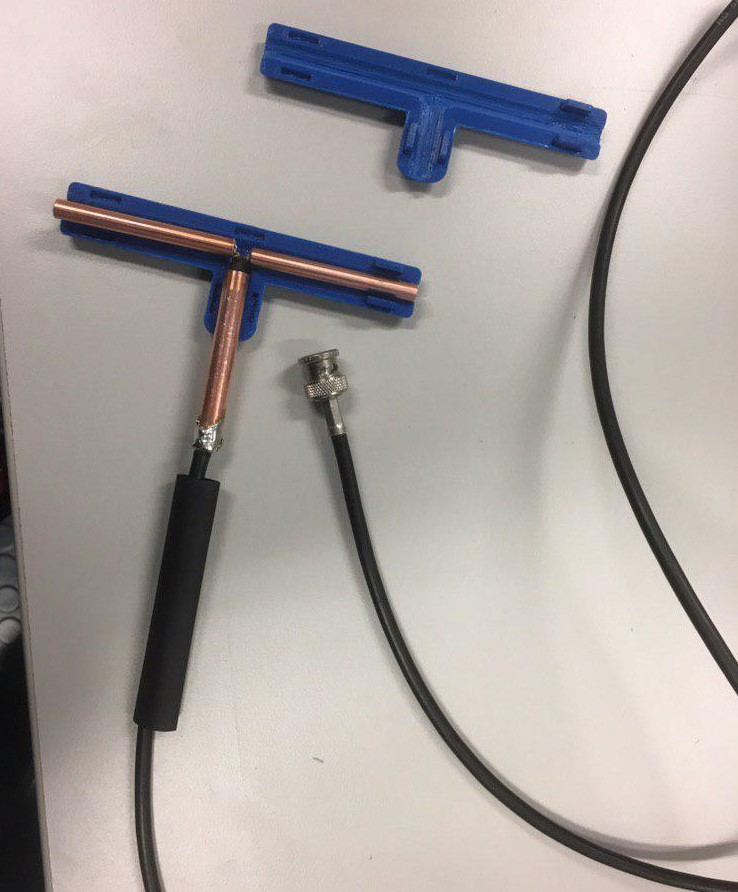
\includegraphics[scale=0.35, trim={0cm 12cm 0cm 0cm}, clip]{Bilder/Ant_innen_1}
	\caption{Aufbau der ersten gebauten Antenne mit Antennengehäuse und Innenleben. Zu sehen sind die beiden sendenden parallelen Röhrchen, sowie das dazu orthogonale Röhrchen, dass als Balun fungieren sollte. Am unteren Bildrand ist noch der vorbereitete Schrumpfschlauch und das ende des Kabels zu sehen.}
	\label{Antenne1}
\end{figure}
Mit den ersten zwei fertigen Antennen wurden erste Probemessungen gemacht um zu sehen ob in dem erwarteten Frequenzbereich ein Intensitätsmaximum zu finden war. Jedoch konnte man im erwarteten Frequenzband nichts auffallendes erkennen. Auffällig war nur ein unregelmäßig auftauchender Peak bei einer Frequenz von $2.4\,$GHz, den wir stark für das WLAN Signal halten. Außerdem konnte man auch andere Peaks (vermutlich Bluetooth und Mobilnetz) erkennen wenn Handys in der nähe der Antenne waren. Somit hatten wir zumindest Funktionierende Antennen die Signale empfangen konnten. Allerdings konnten wir noch nicht wie gewünscht auf einer bestimmten Frequenz senden und dieses Signal messen.

\subsection{Tag 2}

Am nächsten Tag wurden weiter versucht, das Hack-RF zum laufen zu bringen. Leider startete der RaspberryPi nicht mehr, sodass der gestrige Installationsprozess über Nacht erneut durchgeführt werden musste.\par
Außerdem wurden die Antennen weiter getestet. Eine mögliche Lösungen für das Problem mit dem Senden war die Entfernung des Gehäuses, was aber zu keinen besseren Ergebnissen geführt hat. Auch andere Positionen im Raum führten zum selben Ergebnis, dass kein besonderes Intensitätsmaximum empfangen wurde. Es machte sich jedoch schnell bemerkbar, dass der Raum einem Resonator entspricht und kleine Änderungen im Aufbau des Raum größere Unterschiede bezüglich der Übertragenen Leistung machte. Deshalb haben wir alle Tische und Stühle zur Seite geschoben und bei zukünftigen Messungen weder Geräte noch unsere Positionen verändert um stets die selben Bedingungen zu haben.\par
Da kein Messgerät zur Messung der Antennengüte vorhanden war, wurde versucht durch auftragen der maximalen empfangenen Leistung in Abhängigkeit der Frequenz ein Peak zu ermitteln. Hierbei wurde für über einen längeren Zeitraum die maximale Intensität zu jeder Frequenz aufgenommen. Da diese Messungen auch nicht aufschlussreich waren, wurde versucht das Stehwellenverhältnis (SWV oder ``standing wave ratio'' SWR im englischen) mittels des Spectrum-Anaylzers zu bestimmen. Leider war dies erfolglos, da wir zu diesem Zeitpunkt keinen Richtkoppler zur Verfügung hatten.

\subsection{Tag 3}

Am Mittwoch war das Hack-RF vollständig einsetzbar, es wurde nun mit einem anderen RaspberryPi betrieben. Das Hack-RF nutzten wir um eine erste Polarisationsmessungen durchzuführen. Auch hier zeigte sich, dass Bewegung von Personen im Raum oder das öffnen eines Fensters die Messwerte stark beeinflusste. Im laufe des Tages erhielten wir einen Richtkoppler, mit welchem die Güte der Antenne gemessen werden konnte. \textcolor{red}{Erik evtl. nochmal erläutern}\par
Hier stellte sich heraus die Antennen insgesamt eine sehr Ineffektive Charakteristik hatten und auf keinem Frequenzband relativ effizient sendeten. Da zusätzlich ein Wackelkontakt bei einer der Antennen auftrat, wurden zwei neue mit einem Optimierten Design erstellt. Hierbei wurde kein drittes Kupferrohr als Balun senkrecht zum Dipol eingesetzt, sondern die beiden Arme der Antenne direkt an eine BNC-Buchse gelötet, wie in Abbildung \ref{Antenne2} zu sehen ist.\par
Beim Test der neuen Antennen zeigte sich eine deutliche Verbesserung zur ersten Generation. Durch den Spectrum Analyzer mit Richtkoppler konnte recht genau gezeigt werden, dass unsere Antennen im erwarteten Bereich besonders gut senden können (die Tiefsten Dips auf den Abbildungen \ref{Ant1} und \ref{Ant2}).\textcolor{red}{Bild: sind das die richtigen Bilder} Da beide trotzdem leichte Unterschiede in der Peak-Frequenz hatten, wurde die Frequenz eine mithilfe eines Kondensators an der schlechteren Antenne getrimmt, um sie der Peak Frequenz der besseren Antenne anzunähern. Das Endergebnis ist auf Abbildung \ref{Ant2-getrimmt} dargestellt. Da das Bild leider schlacht zugeschnitten ist, und der Marker nicht auf der Peakfrequenz liegt sind noch einmal die Frequenz-Charakteristiken der beiden Antennen (und bei Antenne 2 nach dem trimmen) in Abbildung \ref{Vergleich} dargestell.\textcolor{red}{Bild: so okey ?} 

\subsection{Tag 4}

Mit den nun aufeinander abgestimmten Antennen wurde beschlossen, sich auf eine  Polarisationsmessung und Abstandmessung zu beschränken und die Messung der Strahlungscharakteristik wegzulassen. Da jedoch auffällig war wie Problematisch die Umgebung des Labors war, wurden diese Messungen im Labor so wie im Garten der Physik und am Parkplatz vor dem Westbau durchgeführt.

\subsection{Tag 5}

Am letzten Tag wurden noch zusätzliche Messungen zum Abstand und zur Polarisation im Großen Hörsaal durchgeführt. Da die Messungen im Labor bis dahin wegen Bewegung von Personen sehr ungenau waren wurde hier nochmal eine Messung durchgeführt, um zu zeigen wie groß die Schwankungen sind und eine Messung bei der sich im Labor wirklich nichts verändert und sich niemand Bewegt. \textcolor{red}{Messung? Unterkapitel mit Bildern und etwas Text da häufig erwähnt !!!}
Anschließend wurden noch weitere Richtkoppler der Werkstatt getestet, ob diese sich wie der geliehene verhielten.
\begin{figure}[ht]
	\centering
	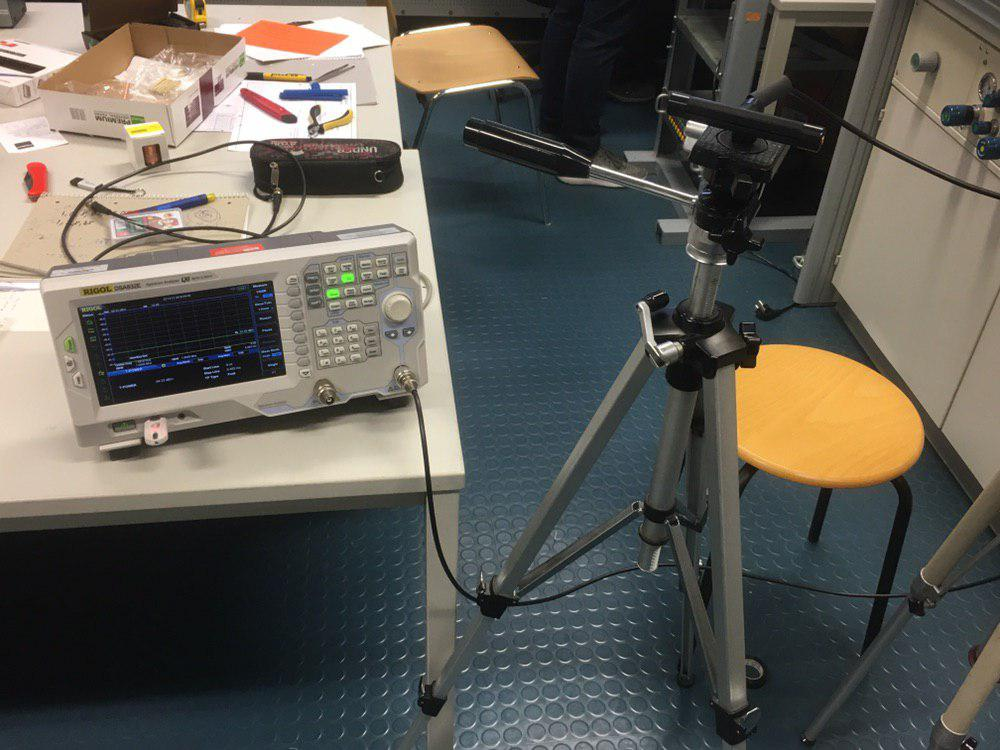
\includegraphics[scale=0.35, trim={0cm 8cm 3cm 2cm}, clip]{Bilder/Ant_Fktgen}
	\caption{Gebaute Antenne auf dem Stativ an den Spektrum-Analyzer angeschlossen. Bei einer Messung wurde die zweite Antenne an den Input angeschlossen und die Intensität des empfangenen Signals bei verschiedenen Frequenzen gemessen.}
	\label{ersteMessung}
\end{figure}
\begin{figure}[ht]
	\centering
	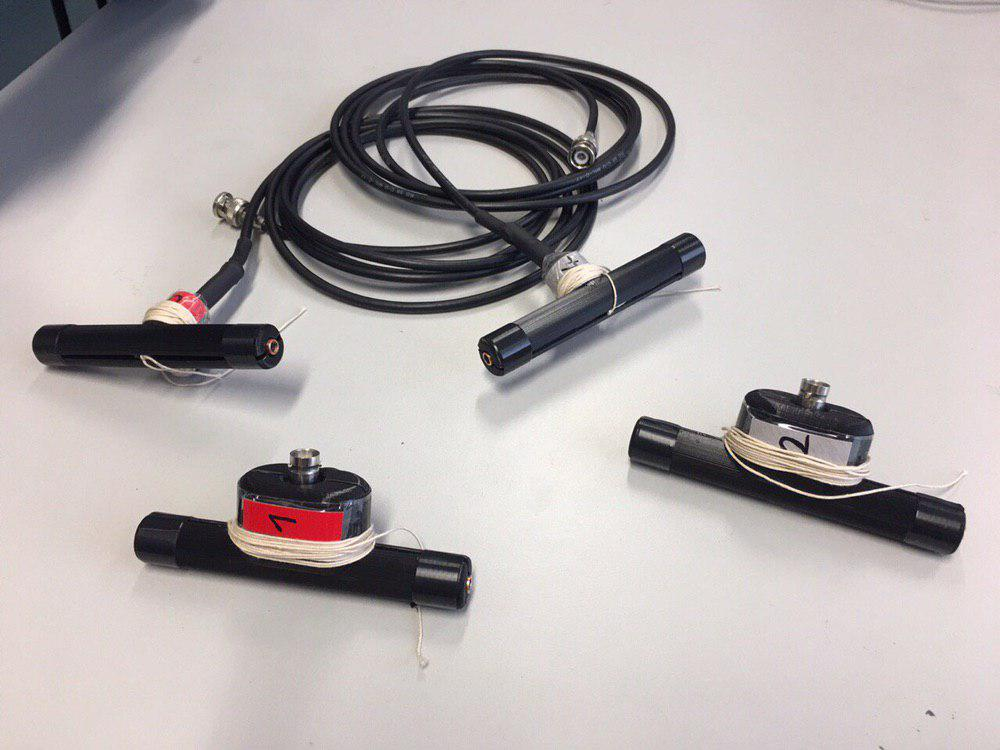
\includegraphics[scale=0.3, trim={0cm 3cm 0cm 1cm}, clip]{Bilder/Ant_12}
	\caption{Beide Antennen Generationen nebeneinander. Hinten die erste Generation vorne die 2.Generation. Die erste Generation Antennen hatten den Nachteil fest an Kabel gebunden zu sein, und einen integrierten Balun zu haben, der nicht wie erwartet funktionierte. Die neuen Antennen haben einen Standardisierten BNC-Anschluss und keinen Balun mehr. Außerdem sind die Gehäuse verbessert und besitzen eine Stativ-Halterung.}
	\label{Antennen1u2}
\end{figure}
\begin{figure}[ht]
	\centering
	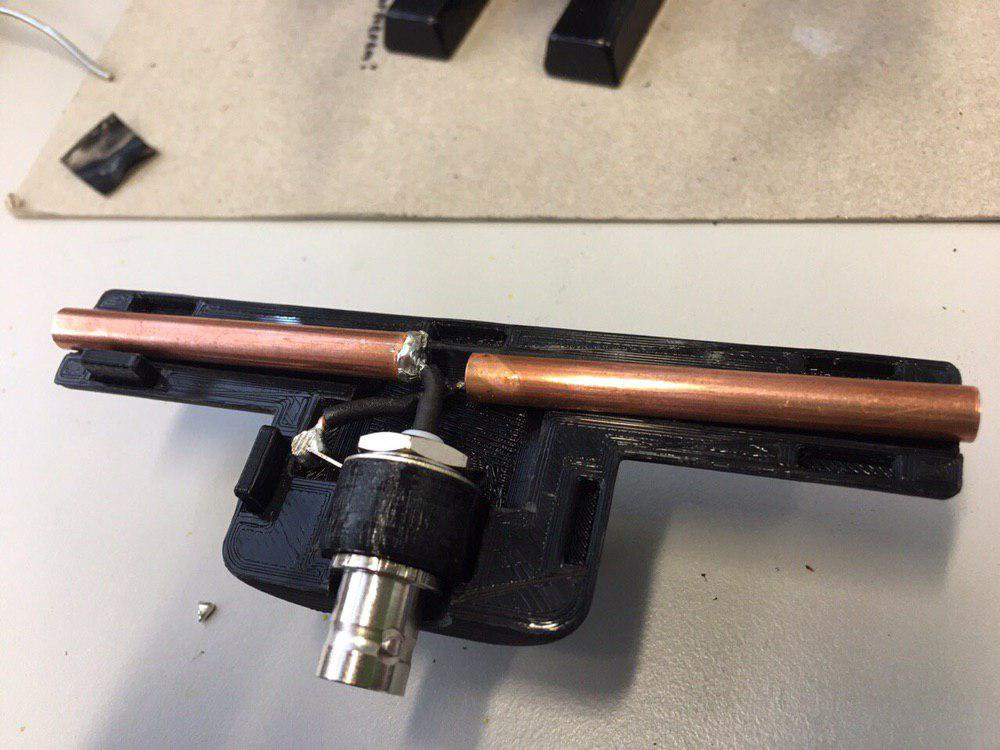
\includegraphics[scale=0.4, trim={0cm 0cm 0cm 8cm}, clip]{Bilder/Ant_innen_2}
	\caption{Innerer Aufbau der 2.Antennengeneration. Man sieht die beiden Kupferröhrchen angelötet an zwei Kabel, welchen an die BNC-Stecker Buchse gelötet wurden. Das Gehäuse sorgt nur für Stabilität, und parallele Ausrichtung der Röhrchen.}
	\label{Antenne2}
\end{figure}


\textcolor{red}{Bilder \ref{ersteMessung}, \ref{Antennen1u2}, \ref{Antenne1} und \ref{Antenne2} refferieren !!!}


\section{Details zu den verwendeten Antennen}

\subsection{Antennenbau}

\subsubsection{Erste Generation}

Die erste Antennengeneration wurde nach der Anleitung \cite{Antennenbauanleitung} vom Akademisk Radioklubb gebaut. Diese bestand aus drei $55\,$mm langen Kupferrohren mit einer Wandstärke von $1\,$mm. Hiervon wurden zwei der Rohre, wie bei einem Dipol erwartet, nebeneinander an Kern und Abschirmung eines halbierten Koaxialkabels mit BNC Buchse gelötet. Das dritte Rohr wurde etwas unterhalb der beiden Antennenarme am Kabel als Balun zur Wandlung zwischen dem voraussichtlich asymmetrischen gesendeten Signal und dem symmetrischen Dipolfeld angelötet. Diese Antennen sind auf Abbildung \ref{Antenne1} zu sehen.

\subsubsection{Zweite Generation}

 Diese haben im Gegensatz zu dem alten Modell keinen Balun (bestehend aus einer Kupferröhre um Signalkabel) mehr.\par
Die Antennen bestehen also nur aus zwei $55\,$mm langen Kupferrohren, die jeweils an Leitung und Schirm eines BNC Gehäuseanschlusses gelötet wurden. Diese Konstruktion wird in einem 3D-gedruckten Gehäuse montiert, sodass die Röhrchen parallel zueinander und orthogonal zum Signalkabel sind. Der nun im Gehäuse eingebaute BNC Anschluss kann nun wie sonst üblich mit kompatiblen Geräten (Oszilloskop, Spectrum Analyzer, etc.) verbunden werden. Dieses Design ist also nicht mehr an ein Kabel gebunden, was den Vorteil hat, dass die Länge variabel ist und ein schlechtes Kabel schnell und leicht ausgetauscht werden kann.\par
Die Plastikgehäuse wurden absichtlich so designet, dass sie ohne Metallteile zusammengebaut werden könnte, da diese die Strahlungscharakteristik beeinträchtigen könnten. Der Kunststoff selbst ist sehr dünn und schien keinen Einfluss auf die Messungen nehmen, dies haben wir rein qualitativ überprüft, indem wir das empfange Signal ohne sowie mit Gehäuse verglichen haben und keinen unterschied feststellen konnten.\par
Außerdem haben die Gehäuse eine Befestigung mit Stativ-Gewinde, sodass sie an Standartmäßigen Fotokamera-Stativen befestigt werden können. Die neuen Antenne sind auf den Abbildungen \ref{Antennen1u2} und \ref{Antenne2} zu sehen.

\subsection{Messung der Antennengüte}
Um die Frequenzen, bei welchen unsere gebauten Antennen relativ gut senden und empfangen können zu bestimmen, wurde die reflektierte Leistung der Antennen für verschiedene Frequenzen bestimmt. Hierzu wurde mithilfe des Spectrum Analyzers ein Frequenzbereich von einigen MHz bis zu $3\,$GHz auf die Antennen gesendet. Dieses Signal wurde dann über einen Richtkoppler auf die zu testende Antenne geleitet, welche dann einen Teil des Signals abstrahlt oder in die Leitung reflektiert. Dieser reflektierte Teil wird über den Richtkoppler zur Messung ausgekoppelt. Beim vermessen der Antennen muss zusätzlich die Charakteristik von Kabeln und dem verwendeten Richtkoppler berücksichtigt werden, worauf wir aber leider nicht genauer eingehen können. Die in diesem Zusammenhang erhobenen Daten befinden sich in der angefügten Messwertesammlung. Zur Bestimmung charakteristischer Frequenzbänder haben wir nur einen Ausgleich mittels des Spectrum Analyzers vorgenommen, welcher die reflektierte Leistung des Richtkopplers und einer $50\,\Omega$  Dummyload normalisierte. Somit erhielten wir für unsere Zwecke brauchbare Charakteristiken. 
\textcolor{red}{Bild Beispielcharakteristik}
\textcolor{red}{Bild Aufbau}

\subsection{Vergleich der Antennen}
Wie im vorherigen Abschnitt besprochen haben wir die Charakteristiken der vier Antennen aufgenommen und verglichen.
\textcolor{red}{Bilder der 4 Messungen "ant 1... ant4" oder so}
Hierbei wurde deutlich, dass die Antennen erster Generation eine komplett andere Charakteristik aufweisen als erwartet, wogegen die Antennen der zweiten Generation sich erwartungsgemäß verhalten. Aufgrund des dipolartigen Aufbaus der Antennen wurde ein relativ breiter Bereich von Resonanz erwartet mit einigen Resonanzen bei Vielfachen der ursprünglichen Resonanzfrequenz. Wie aus den Bildern entnehmbar ist, kann dieses Verhalten nur bei Antennen zweiter Generation beobachtet werden, die vorherigen haben kein klares Minimum an reflektierter Leistung.


\subsection{Trimmen der Empfangsantenne}
Wie in den Bildern zur Reflektionscharakteristik der zweiten Generation Antennen ersichtlich, besitzen beide ein Leistungsminimum in einer Ähnlichen Region. Antenne 2 war das Reflektionsleistungsminimum jedoch deutlich von der Zielfrequenz bei ca. $1.3\,$GHz abgewichen, sodass wir uns entschieden die Impedanz der Antenne auf das richtige Band zu trimmen. Da wir eine relativ feine Anpassung vornehmen wollten, entschieden wir uns variable Kondensatoren parallel zu den Antennenarmen schalten. Wir erhielten drei verschiedene Drehkondensatoren, wobei der mit größter Kapazität am ende verwendet wurde. An diesen wurden zwei Kabel gelötet und an die Antennenarme gedrückt. Nach einigem Herumprobieren entschieden wir uns für eine Position ca. $\frac{2}{3}$ der Stablänge gesehen von den Lötstellen aus. Wir bemerkten, dass die eingestellte Kapazität des Drehkondensators kaum eine Auswirkung auf die Charakteristik hatte, aber die Positionsänderung der Drähte einen großen Einfluss hatte. Vermutlich ist dies durch die Induktivität der Kabel erklärbar. Die induktive Impedanz steigt linear mit der Frequenz, während die kapazitive mit steigender Frequenz fällt. 
\textcolor{red}{Bild der getrimmten Antenne: Aufbau, Vorher nachher chara}

\subsection{Vergleich der Richtkoppler}
Es wurden zusätzlich zum Richtkoppler, mit welchem wir die Messungen zur Antennengüte und das Trimmen durchführten, weitere Richtkoppler bereitgestellt. Als diese nach oben beschriebenen Verfahren zur Messung der nicht getrimmten Antenne der zweiten Generation verwendet wurden, wurde eine völlig unterschiedliche Charakteristik angezeigt. Etwa als würde die Antenne nahezu das gesamte Signal reflektieren. Dies kann aber nach den geglückten Fernfeldmessungen nicht der Fall sein.
\textcolor{red}{Bild Vergleich Richtkoppler}

\section{Versuchsaufbau und Durchführung der Messungen}
\label{Versuchsaufbau} 

\subsection{Die Antennen}

Für die ausgewerteten Messungen haben wir nun ausschließlich die neuen Antennen verwendet. Es existieren quantitative Messungen mit den Antennen erster Generation, jedoch fehlte die Zeit auch diese auszuwerten.

\subsection{Versuchsaufbau Abstandsmessung}

Für die jeweiligen Messung haben wir die beiden Antennen an Stativen befestigt und gegenüber voneinander platziert. Die Gehäuse der Antennen wurden an einer dafür vorgesehenen Öse mit einer Schnur verbunden, um die Parallelität der Antennen bei der Anstandsmessung beziehungsweise einen akkuraten Winkel bei der Polarisationsmessung zu gewährleisten.\par
Beide Antennen wurden an den Spectrum Analyzer angeschlossen. Der Spectrum Analyzers sendet nun nacheinander Signale mit verschiedenen Frequenzen durch das gesamte Frequenzband des Spectrum-Analyzers an die Sender-Antenne und zeichnet die Intensität des von der Empfänger-Antenne kommenden Signals auf.\par
Ein Vorteil an dieser Messung gegenüber dem Senden einer Frequenz über das Hack-RF ist, das wir so auch leicht Störsignale, die von der Antenne empfangen werden feststellen können und damit ausschließen können, dass wie so ein Störsignal mit in die Messung einbeziehen. Hierbei sind Störsignale wie z.B. WLAN oder andere zeitlich nicht konstante Funksignale gemeint.

\subsection{Versuchsaufbau Polarisationsmessung}

Zur Messung der Polarisation wurden die Beiden Antennen in einem festen Abstand voneinander auf dem jeweiligen Stativ befestigt. Zur Bestimmung des Winkels der Antennen zueinander, wurde ein Faden genutzt der zwischen beiden Antennen gespannt wurde. Danach konnte man mit Hilfe eines Geodreiecks den gewünschten Winkel zwischen Antenne und Faden einstellen. Sender und Empfänger wurden dann an den Spectrum-Analyzer angeschlossen.

\subsubsection{Durchführung}


Während den Messungen saßen eine oder zwei Personen am Spectrum-Analyzer, und damit in Nähe der Antennen um die Messwerte abzulesen. Die anderen bei der Messung anwesenden haben entweder den Abstand oder für die Polarisationsmessung den Winkel der empfänger-Antenne verändert und sich dann wieder vom Versuchsaufbau entfernt.\par
Dieser Abstand beziehungsweise Winkel wurde dann Notiert und die am Spectrum-Analyzer abgelesene Leistung in dBm protokolliert.

\section{Auswertung}
Bei der Auswertung unserer Messwerte haben wir uns auf die Abstandsmessungen und die Polarisationsmessungen mit den Antennen zweiter Generation beschränkt. Hierzu werden wir beispielhaft sowohl eine Abstandsmessung als auch eine Polarisationsmessung auswerten. Die restlichen Ergebnisse sind im Anhang zu finden und werden dann im Abschnitt  ,,Diskussion der Ergebnisse`` diese genauer betrachten und interpretieren. \par 
Zuerst betrachten wir die Abstandsmessungen im Großen Hörsaal.Dazu prüfen wir nun ob unsere Messungen sich im Fernfeld oder im Nahfeld der Sendeantenne bewegt. Hier nutzen wir die Näherung:
\begin{equation}
r_{\tx{ff}} \geqslant 2\cdot\lambda
\label{rff}
\end{equation}
Damit ist gemeint ab $r_{\tx{ff}}$ beginnt das Fernfeld. Jedoch ist das nur eine Näherung. Tatsächlich ist der genaue Übergang zwischen Fern- und Nahfeld keine eindeutige Grenze sondern dazwischen liegt der Übergangsbereich, welcher die Abgrenzung zwischen Nahfeld und Fernfeld erschwert. Jedoch soll für unsere Abstandmessung diese Näherung ausreichend sein, da, wie man gleich sehen wird, wir uns bei dem meisten Messwerten mit Sicherheit im Fernfeld bewegen. \par 
Um nun $r_{\tx{ff}}$ für unsere Sendeantenne zu berechnen, berechnen wir zunächst die Wellenlänge $\lambda$ für unsere Sendefrequenz $f=1{,}616\,$GHz mit einem Ablesefehler von $\Delta f=0{,}0005\,$GHz ($c\approx 3\cdot10^{8}\,\frac{\tx{m}}{\tx{s}}$). Damit erhalten wir für die Wellenlänge und den Fehler (mittels Gauß'scher Fehlerfortpflanzung) folgende Werte:
\begin{equation*}
\lambda = \frac{c}{f} \approx 0{,}1856\,\tx{m} \qquad \qquad
\Delta \lambda = \frac{\Delta f c}{f^{2}} \approx 1{,}1 \cdot 10^{-4}\,\tx{m}
\end{equation*}
Somit erhalten wir für das Fernfeld einen Mindestabstand von: 
\begin{equation*}
r_{ff} \geqslant 2\cdot\lambda = 0{,}3713\,\tx{m}\, \pm 2\cdot10^{-4}\,\tx{m}
\end{equation*}
Somit können wir sagen wir bewegen uns bei unseren Abstandsmessungen im Fernfeld, da bei allen Messungen höchstens ein bis zwei Werte unter $r_{\tx{ff}}$ liegen (siehe Messwerte im Anhang). \par 
Als nächstes berechnen wir die Leistung der Messwerte in W, da sie noch in dBm angegeben sind. Dazu nutzen wir die Formel:
\begin{equation}
\tx{I in Watt}: 10^{\frac{(I[\tx{dBm}]-30)}{10}}
\label{w}
\end{equation}
Die Fehler haben wir auf Grund der Schwankungen des Messpunktes auf $\Delta I=$$\pm 1\,$dBm geschätzt. Damit ist dieser Fehler deutlich größer als die aus den Impedanzen des Spectrum Analyzers (aus den Herstellerinfos), so das wir diese vernachlässigen können. Da diese Fehler auf Grund der logarithmischen Messwerte asymmetrisch sind, und wir aber gleich große Fehler in beider Richtungen haben wollen, rechnen wir:
\begin{equation*}
I_{+1} := I+1\,\tx{dBm} \quad\tx{,}\,I_{-1} := I-1\,\tx{dBm} \quad \Rightarrow\tx{in Watt umrechnen mit \eqref{w}} \quad \Rightarrow 
\end{equation*}
\begin{equation}
\Delta I = \frac{(I-I_{-1})+(I_{+1}-I)}{2}
\label{deltaI}
\end{equation}
Wir bilden also den Mittelwert aus den zwei ungleich großen Fehlern. Dies zeigen wir nun für den Wert $I=-38{,}85\,\tx{dBm} \approx$ $1{,}3031\cdot10^{-7}\,$W (GrH Messung 1: $d=120\,$cm):
\begin{equation*}
I_{+1} = -37{,}85\,\tx{dBm} \approx 1{,}6405\cdot 10^{-7}\,\tx{W} \qquad I_{-1} = -39{,}85\,\tx{dBm} \approx 1{,}0351\,\tx{W}
\end{equation*}
\begin{equation*}
\Delta I = \frac{(I-I_{-1})+(I_{+1}-I)}{2} \approx 0{,}9 \cdot10^{-7}\,\tx{W}
\end{equation*}
Somit ist $ I = (1{,}3 \pm 0{,}3) \cdot 10^{-7} \, \tx{W} $.

\subsection{Abstandsmessung}

Nach dem wir alle Werte berechnet haben, tragen wir die Leistung $I$ in Abhängigkeit des Abstandes $d$ auf. Wie bereits zu erkennen ist, entsprechen die Messwerte ca. einem $\frac{1}{d^{2}}$ Verlauf, welchen wir für die Leistung im Fernfeld erwarten würden. Man sieht die Werte Fallen am Anfang sehr Stark und nähern sich dann der Null an. Um quantitative Aussagen über den Verlauf machen zu können, versuchen wir nun eine $\frac{1}{d^{2}}$-Funktion an unsere Messwerte zu fitten.

\begin{figure}[ht]
	\centering
	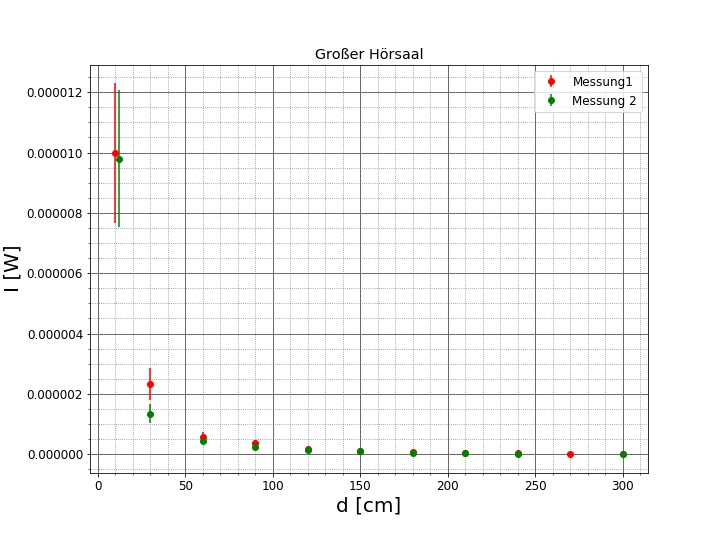
\includegraphics[scale=0.45]{Bilder/bsp}
	\caption{Gemessenen Intensität in Abhängigkeit vom Abstand $d$. Auf der $y$-Achse ist die empfangene Intensität in Watt und auf der $x$-Achse der Abstand zur Sendeantenne in cm.}
	\label{Abstand-bsp}
\end{figure}

\FloatBarrier

\noindent
Als nächstes nutzen wir die Python-Funktion \verb|curve_fit| \cite{curvescipy} Funktion um eine Funktion mit dem erwarteten $\frac{1}{d^{2}}$ Verlauf zu finden. Dazu nutzen wir:
\begin{equation}
f(d) = a + \frac{b}{d^{2}}
\label{f}
\end{equation}	
Hierbei sind $a$ und $b$ freie Parameter, welche \verb|curve_fit| an die Messwerte anpasst und $d$ der Abstand zur Sendeantenne. Zusätzlich wählen wir nun wieder eine logarithmische Skala für die $y$-Achse, um Messwerte, welche gegen Null gehen besser unterscheiden zu können. Dies ergibt (wieder mit den Messwerten aus dem großen Hörsaal) den Graphen Abbildung \ref{GrH-A}.

\begin{figure}[ht]
	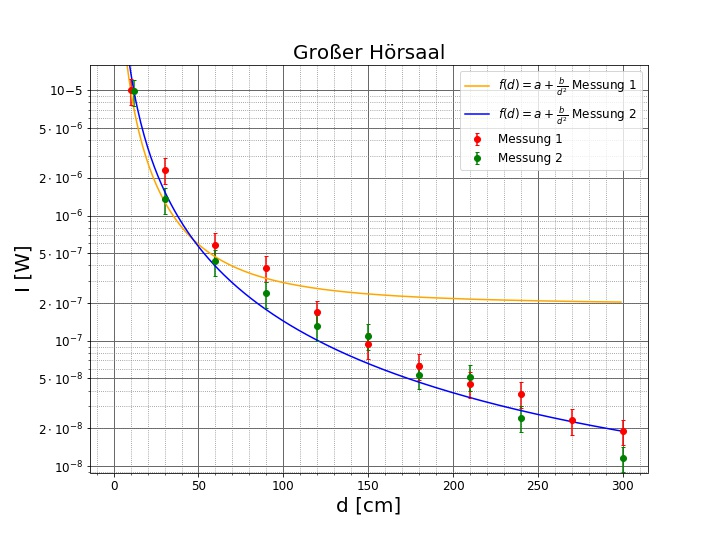
\includegraphics[scale=0.55]{Bilder/Abstand-GrH.jpg}
	\centering
	\caption{Gemessenen Intensität in Abhängigkeit vom Abstand $d$ im großen Hörsall der Physik. Auf der logarithmischen $y$-Achse ist die empfangene Intensität in Watt aufgetragen und auf der $x$-Achse der Abstand zur Sendeantenne in cm. Zusätzlich sind Fehler in $y$-Richtung nach Formel \eqref{deltaI} eingetragen. Die Fehler in $x$-Richtung $\Delta d = 2\,$cm sind zu klein und deswegen nicht eingezeichnet. Auch wurde die Funktion $f(d)$ \eqref{f} mittels \texttt{curvefit}. (Python Modul \cite{curvescipy}) an die Messwerte geplottet.}
	\label{GrH-A}
\end{figure}
\FloatBarrier
Bei diesen Messwerten ergeben sich für die Parameter $a$ und $b$ die Werte:
\begin{equation*}
\tx{Messung 1:} \quad a = (1{,}9\pm1{,}2)\cdot10^{-7}\,\tx{W} \quad b = (9{,}9\pm0{,}4)\cdot10^{-4}\,\tx{Wcm}
\end{equation*}
\begin{equation*}
\tx{Messung 2:} \quad a = (0{,}3\pm2{,}8)\cdot10^{-8}\,\tx{W} \quad b = (1{,405\pm0{,}013})\cdot10^{-3} \,\tx{Wcm}
\end{equation*}
Wir werden jedoch bei den anderen Messwerten und den dazugehörigen Funktionen diese Parameter nicht weiter betrachten, da wir uns auf Grund der begrenzten Auswertungszeit nur auf den $\frac{1}{x^{2}}$ Verlauf beschränken werden. Nun nur ein paar kurze Worte zu ihnen. Der Parameter $a$ sollte idealerweise Null sein und ist auch bei allen Messwerten sehr klein, mit Werten zwischen $10^{-7}\,$W und $10^{-9}\,$W. Zum Parameter $b$ ist nochmals zu erwähnen, dass wir davon ausgehen, dass wir uns während unserer gesamten Messung im Fernfeld bewegen. Deswegen können unsere Funktionen eigentlich nur bis zu einen Abstand von ca. $r_{\tx{ff}}=(37{,}13\pm0{,}02)\,$cm (nur eine Näherung! Siehe \eqref{rff}) richtige Vorhersagen treffen.  \par 
Deswegen werden wir auf den Parameter $b$ in dieser Auswertung nicht eingehen.

\subsection{Polarisationsmessung}

Als nächstes betrachten wir die zwei Polarisationsmessungen. Auch hier werden wir beispielhaft die Auswertung der Messung im großen Hörsaal betrachten. \par 
Als erstes rechnen wir die Werte wieder in Watt mittels Formel \eqref{w} um. Auch wird der Fehler wieder in gleicher Weise wie zuvor mit der Formel \eqref{deltaI} bestimmt. Danach tragen wir die Intensität in Abhängigkeit vom Winkel auf. \par 
Nach der Theorie erwarten wir folgenden Verlauf der Polarisation:
\begin{equation}
I(\phi) = I_{max}\cdot \cos^{2}(\phi)
\label{I}
\end{equation}
Also versuchen wir nun zuerst eine $\cos^{2}$ Funktion mit mehreren Parametern einzubauen. Diese hat die Folgende Form: 
\begin{equation}
I_{1}(\phi) = a \cdot \cos((b \cdot\phi) - c)^{2} + d
\label{I1}
\end{equation}
Wobei wir hier nach Formel \eqref{I} erwarten würden, dass $a=I_{0}$, $b=1$, $c=0$ und $d=0$ ist. Dies ist bei uns jedoch nicht der Fall. Eventuelle Gründe dafür werden im nächsten Abschnitt ,,Diskussion `` besprochen. \par 
Nun wollen wir noch einen zu erwarteten Verlauf nach Formel \eqref{I} einzeichnen. Dazu wählen wir unser $I_{max}=I(0)$ und erhalten dann:
\begin{equation}
I_{2}(\phi) = I(0)\cdot \cos^{2}(\phi)
\label{I2}
\end{equation}


\section{Diskussion}

\subsection{Fehlerquellen}

Bei den Messungen gab es eine Reihe an Fehlerquellen. Hierbei hatten wir als erstes als statistische Fehler, Fehler der Abstands und Winkelmessung. Hierbei haben wir einen allgemeinen Fehler für den Abstand auf $2$\,cm geschätzt und den Fehler für die Winkel auf $2^{\degree}$. Auch für die Frequenz und der dort gemessenen Leistung haben wir einen statistischen Fehler. Hierbei wurde die Frequenz auf $0.001\,$GHz und die Leistung auf $1$\,dBm geschätzt. Zusätzlich konnte es passieren das unsere Antennen bei der Abstandsmessung leicht verschoben zueinander lagen. Dies ist bei der Abstandsmessung im Gegensatz zur Polarisationsmessung ein statistischer Fehler, da hier Verschiebung der beiden Antennen sich durch das neu Aufstellen zufällig ändern kann.
Bei der Winkelmessung ist dies ein Systematischer Fehler da dieser bei jeder Messreihe konstant blieb. Dafür kommt hier noch ein Fehler dazu der durch das Drehen der Antenne zustande kam. Hierbei wurde die Antenne aufgrund der Aufhängung nicht um den Antennenmittelpunkt sondern um einen Punkt etwas weiter hinten gedreht wodurch sich der Abstand so wie die Verschiebung der Antennen zueinander systematisch geändert hat. Ein weitere systematische Fehler ist, dass die Werte stark durch unsere Umgebung beeinflusst wurden. Oft hat hier die Umgebung als Resonator fungiert und unsere Werte abhängig von der Umgebung beeinflusst hat. Der Ort der Messung hat auch unser Hintergrundrauschen beeinflusst da dieses je nach Ort unterschiedlich stark abgeschirmt wurde. An dieser stelle kommt jedoch noch ein statistischer Fehler dazu welcher sich auf Zeitlich nicht konstante Hintergrundsignale bezieht. Als letzten systematischen Fehler ist zu erwähnen, dass unsere Stative unabhängig vom Raum sich wegen ihrer Metallenen Beschaffenheit fälschend auf unsere Messergebnisse auswirkten haben.

\subsection{Analyse der Graphen}

\subsubsection{Abstandsmessungen}

Auf Abbildung \ref{Garten-A} ist die Abstandsmessung im Garten der Physik zu sehen. Wie schon im Abschnitt \ref{Versuchsaufbau} beschrieben, haben wir die beiden Antennen auf zwei Stativen gegenüber voneinander Positioniert und bei verschiedenen Abständen $ d $ die bei der empfänger-Antenne ankommende Leistung $ I $ gemessen. Die hier angegebenen Werte für die Leistung wurden bereits aus dBm und Watt umgerechnet.\par
Die Messpunkte sind in blau und die Fehler darauf in rot dargestellt. Es gibt hier sowohl Fehler auf die Leistung als auch auf den Abstand. Die Fehler auf den Abstand sind lediglich zum Teil so klein, dass sie fast nicht erkennbar sind.\par
Die blaue Kurve durch die Messdaten entspricht dem in der Auswertung ermittelten Fit der Form $ f(d) = a + \frac{b}{d^2} $, wobei die Parameter $ a $ als $ y $-Achsen Abschnitt und $ b $ als $ y $-Streckfaktor angepasst wurden.\par
Die $ y $-Achse ist logarithmisch aufgetragen, die $ x $-Achse linear. Aufgrund dieser logarithmischen Skala gibt es solche starken Abweichungen bei den letzten Messpunkten.\par
Man sieht also, dass die Streuung der Messpunkte vermutlich größer ist, als die von uns berechneten Fehler. Dies könnte daran liegen, dass eine Messung gut 15 Minuten andauert und der Strahlungshintergrund nicht konstant ist. Da diese Messung draußen stattgefunden hat, gab es leider keine gute Abschirmung von Störsignalen. Wir wollten dennoch Messreihen draußen erstellen um den Störfaktor eines Raums als Resonator ausschließen zu können.\par
Bei dieser Messreihe haben wir über einen Abstand von 50\,cm bis 300\,cm Intensitäten zwischen $ \approx 5 \cdot 10^{-7} \, \tx{W} $ und $ 10^{-8} \, \tx{W} $ gemessen.\\[10pt]
\noindent
Die Nächste Messung wurde auf dem Parkplatz und in einer zur ersten Messung um $ 90^\circ $ gedrehten Anordnung durchgeführt. Hierbei ging es uns nur darum die Umgebungsfaktoren möglichst bei jeder Messreihe zu verändern, sodass wir konstanten Störungen bemerken können.\par
Die Messreihe ist auf Abbildung \ref{Parkplatz-A} dargestellt. Die einzelnen Messpunkte sind wieder in blau, die Fehler in rot dargestellt. Auch hier ist die $ y $-Achse logarithmisch aufgetragen. Die blaue Kurve ist wieder ein $ \frac{1}{d^2} $ Fit mit den Parametern $ a $ und $ b $ wie zuvor. Die Kurve sieht nur aufgrund der logarithmischen Skala so unerwartet aus. Dieser Abfall der Kurve, der hier ab $ 250 \, \tx{cm} $ zu erkennen ist, fällt bei den anderen Messungen nicht auf, da dort der $ y $-Achsen $ a $ positiv ist und die Kurve nicht die $ x $-Achse schneidet. Da der Parameter $ a $ bei dieser Messung als negativ berechnet wurde und in der logarithmischen nur positive Zahlen dargestellt werden, sieht der $ \frac{1}{d^2} $-Verlauf so unerwartet aus.\par
Die Messung wurde genauso durchgeführt wie auch im Garten der Physik. Wie man jedoch sieht haben wir bei dieser Messung bei den gleichen Abständen einen wesentlich größeren Bereich an Intensitäten gemessen. Die Werte gehen von $ \approx 10^{-5} \, \tx{W} $ bis $ \approx 10^{-8} \, \tx{W} $ statt wie zuvor nur von $ \approx 5 \cdot 10^{-7} \, \tx{W} $ und $ 10^{-8} \, \tx{W} $. Wir haben allerdings keine Vermutung, warum die Intensität bei der Messung im Garten der Physik so gering war.\par
Ansonsten fällt noch auf, dass die letzten fünf Messwerte, von denen keiner mit der Kurve verträglich ist, größtenteils unter der Kurve liegen.\\[10pt]
\noindent
Bei der Messung im Labor, die auf Abbildung \ref{Labor-A} dargestellt ist, haben wir wieder einen Verlauf erhalten, der dem erwarteten näher kommt. Die Messdaten sind wieder blau, die Fehler (diesmal nur auf die Intensität, da die auf den Abstand sehr gering waren) in rot und der $ \frac{1}{d^2} $-Fit in blau eingezeichnet.\par
Der Verlauf geht ziemlich gut durch die Messpunkte durch alle Punkte hindurch. Sie liegen gleichmäßig über und unter dem Fit. Auch hier sind vermutlich die Störfaktoren, die die Messpunkte statistisch verschieben wesentlich größer als die Messgenauigkeit unserer Instrumente.\par
Diese Messung war erstaunlich gut dafür, dass wir dabei im Labor waren. Mit den alten Antennen war die Sende- und Empfangscharakteristik so schlecht, dass man im Labor kaum eine große Veränderung Messen konnte. Die Neuen Antenne sind somit also eine sehr große Verbesserung, da die Messwerte nicht nur einem Abfall entsprechen, sondern auch gut an den erwarteten $ \frac{1}{d^2} $-Verlauf passen.\\[10pt]
\noindent
Die letzte Abstandsmessung konnte dann am letzten Tag im Großen Hörsaal durchgeführt werden. Diese hatte insofern ein großes Potential, da wir einerseits in einem relativ gut Abschirmenden Gebäude sind, und die Störfaktoren von draußen hier keine so große Rolle spielen und andererseits die Wände des Raums weit genug entfernt sind, und nicht wie im Labor Stehende Wellen bilden, die die Messung Unvorhersagbar beeinflussen.\par
Die Messdaten sind in Abbildung \ref{GrH-A} dargestellt. Im Großen Hörsaal haben wir zwei Abstandmessungen (wieder in $ 90^\circ $ Ausrichtung zueinander) gemacht, um systematische Störungen durch Reflexionen an den Wänden oder anderen systematischen Fehler


\subsection{Polarisationsmessung}

Die Abbildung 11 zeigt die Polarisationsmessung im Großen Hörsaal. Wie zuvor beschrieben wurde für diese Messung die Sendeantenne für einen festen Abstand von der Empfängerantenne gedreht. In Blau ist die erwartete Intensitätsverlauf von $I(\phi)=I_{max}cos(\phi)$ Die mit den Werten gezeichnete Kurve ist in Orange sichtbar nach rechts verschoben. Dies ist liegt möglicherweise daran, dass der Empfänger leicht gegenüber dem Sender verschoben war wodurch sich auch alle Werte leicht verschoben haben. Auch ist auffallend, dass die orange Kurve nach unten schmaler wird als die Erwartete. Der Grund hierfür könnte sein, dass wir die Antenne nicht um ihren Mittelpunkt sondern um einen Punkt leicht dahinter gedreht haben. Dadurch haben wir zusätzlich noch einen Intensitätsverlust durch die zusätzliche steigende Entfernung der beiden Antennen. D.h wir messen einen schnelleren Abfall bezüglich der Intensität als erwartet. Wenn man sich die blauen Messpunkte anschaut fällt zusätzlich noch auf, dass diese auf beiden Seiten nach einem gewissen Winkel sich kaum merklich verändern. Dies kann daran liegen, dass wir durch denn schnelleren Intensitätsabfall unsere Werte am Ende nicht mehr merklich durch die Drehung ändern weil sie schon fast am Minimum angekommen sind und bis sich die Intensität nach 

\section{Fazit}

erste ANtennen kacke weil kurzschluss

zweite generation besser

1/x**2 gemessen nur mit abweichungen wegen location

polarisation auch gut aber mit winkel offset



\bibliographystyle{plain}
\bibliography{literature}
\addcontentsline{toc}{section}{Literatur}

\section*{Anhang}
\addcontentsline{toc}{section}{Anhang}

\FloatBarrier

\begin{figure}[ht]
	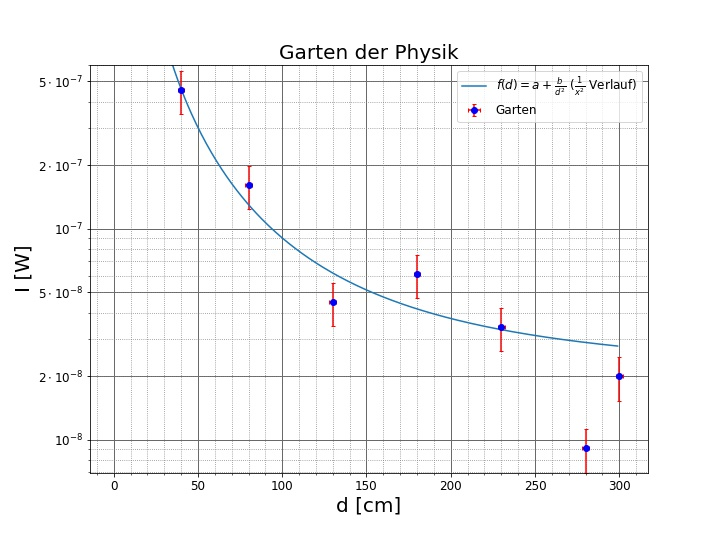
\includegraphics[scale=0.55]{Bilder/Abstand-Garten.jpg}
	\centering
	\caption{Gemessenen Intensität in Abhängigkeit vom Abstand $d$ im Garten der Physik. Auf der logarithmischen $y$-Achse ist die empfangene Intensität in Watt aufgetragen und auf der $x$-Achse der Abstand zur Sendeantenne in cm. Zusätzlich sind Fehler in $y$-Richtung nach Formel \eqref{deltaI} eingetragen. Die Fehler in $x$-Richtung $\Delta d = 2\,$cm sind zu klein und deswegen nicht zu sehen. Auch wurde die Funktion $f(d)$ \eqref{f} mittels \texttt{curvefit}. (Python Modul \cite{curvescipy}) an die Messwerte geplottet.}
	\label{Garten-A}
\end{figure}

\begin{figure}[ht]
	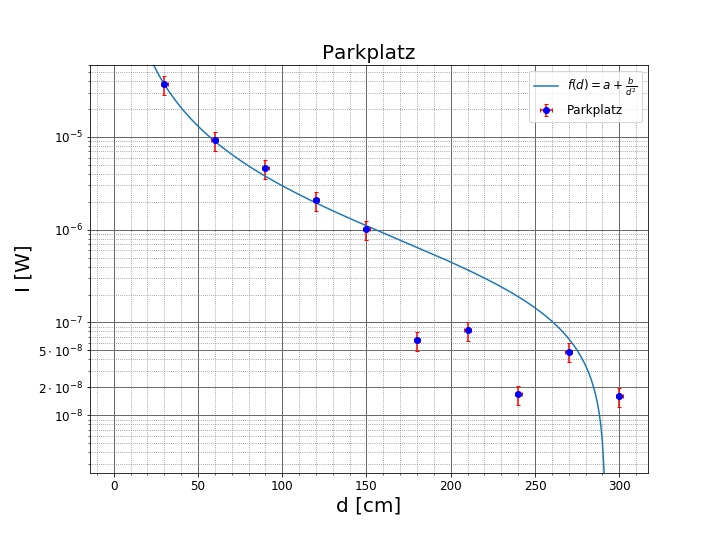
\includegraphics[scale=0.55]{Bilder/Abstand-Parkplatz.jpg}
	\centering
	\caption{Gemessenen Intensität in Abhängigkeit vom Abstand $d$ auf dem Parkplatz. Auf der logarithmischen $y$-Achse ist die empfangene Intensität in Watt aufgetragen und auf der $x$-Achse der Abstand zur Sendeantenne in cm. Zusätzlich sind Fehler in $y$-Richtung nach Formel \eqref{deltaI} eingetragen. Die Fehler in $x$-Richtung $\Delta d = 2\,$cm sind zu klein und deswegen nicht zu sehen. Auch wurde die Funktion $f(d)$ \eqref{f} mittels \texttt{curvefit}. (Python Modul \cite{curvescipy}) an die Messwerte geplottet.}
	\label{Parkplatz-A}
\end{figure}

\begin{figure}[ht]
	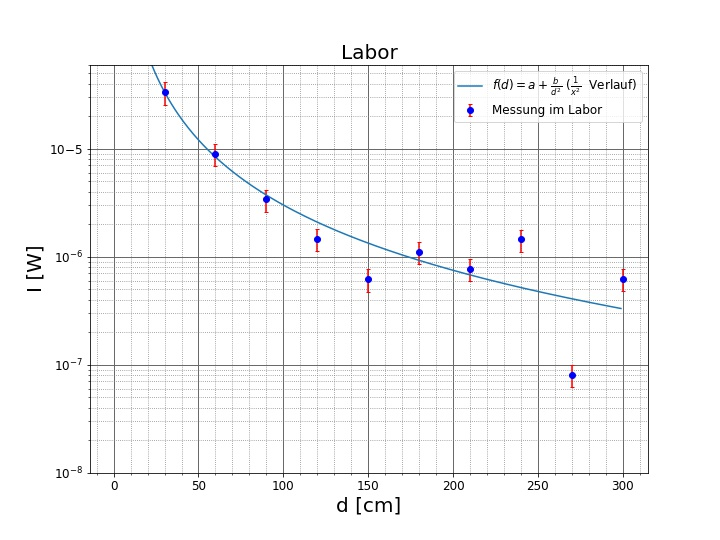
\includegraphics[scale=0.55]{Bilder/Abstand-Labor.jpg}
	\centering
	\caption{Gemessenen Intensität in Abhängigkeit vom Abstand $d$ im Labor. Auf der logarithmischen $y$-Achse ist die empfangene Intensität in Watt aufgetragen und auf der $x$-Achse der Abstand zur Sendeantenne in cm. Zusätzlich sind Fehler in $y$-Richtung nach Formel \eqref{deltaI} eingetragen. Die Fehler in $x$-Richtung $\Delta d = 2\,$cm sind zu klein und deswegen nicht zu sehen. Auch wurde die Funktion $f(d)$ \eqref{f} mittels \texttt{curvefit}. (Python Modul \cite{curvescipy}) an die Messwerte geplottet.}
	\label{Labor-A}
\end{figure}

\begin{figure}[ht]
	\centering
	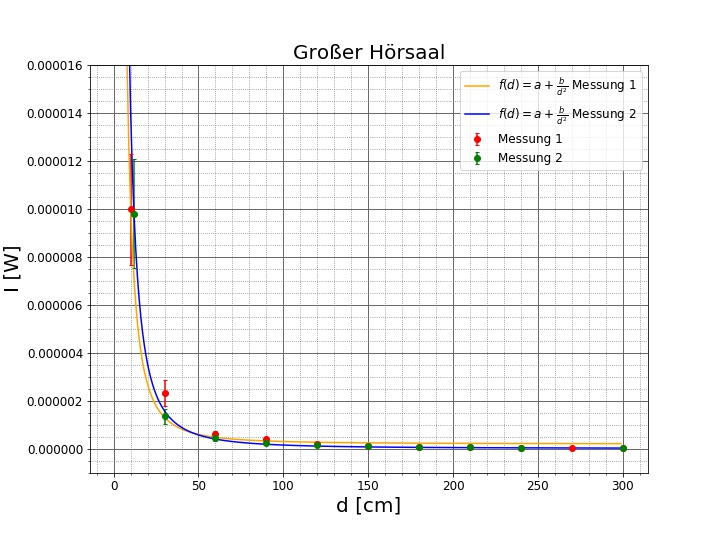
\includegraphics[scale=0.55]{Bilder/bsp2}
	\caption{Gemessenen Intensität in Abhängigkeit vom Abstand $d$ im Großen Hörsaal der Physik. Auf der $y$-Achse ist die empfangene Intensität in Watt aufgetragen und auf der $x$-Achse der Abstand zur Sendeantenne in cm. Zusätzlich sind Fehler in $y$-Richtung nach Formel \eqref{deltaI} eingetragen. Die Fehler in $x$-Richtung $\Delta d = 2\,$cm sind zu klein und deswegen nicht zu sehen. Auch wurde die Funktion $f(d)$ \eqref{f} mittels \texttt{curvefit}. (Python Modul \cite{curvescipy}) an die Messwerte geplottet.}
	\label{Abstand-lin}
\end{figure}

\begin{figure}
	\centering
	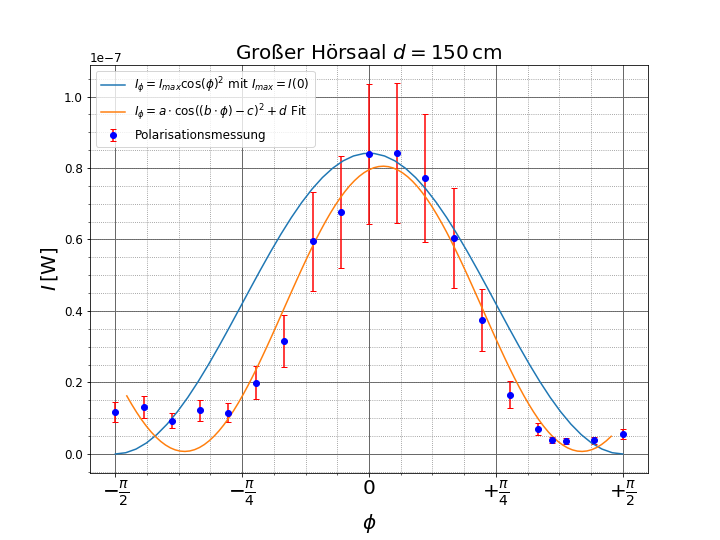
\includegraphics[scale=0.55]{Bilder/Polarisation-GrH}
	\caption{Gemessene Intensität in Abhängigkeit vom Winkel $\phi$ des Empfängers im Großen Hörsaal der Physik. Fehler in $y$-Richtung sind mittels Formel \eqref{deltaI} berechnet und eingetragen. Auch wurde die Funktion $I_{1}(\phi)$ \eqref{I1}  mittels \texttt{curvefit}. (Python Modul \cite{curvescipy}) an die Messwerte geplottet. Auch wurde der theoretische Verlauf nach Formel \eqref{I2} eingetragen.}
	\label{Labor-P}
\end{figure}

\begin{figure}
	\centering
	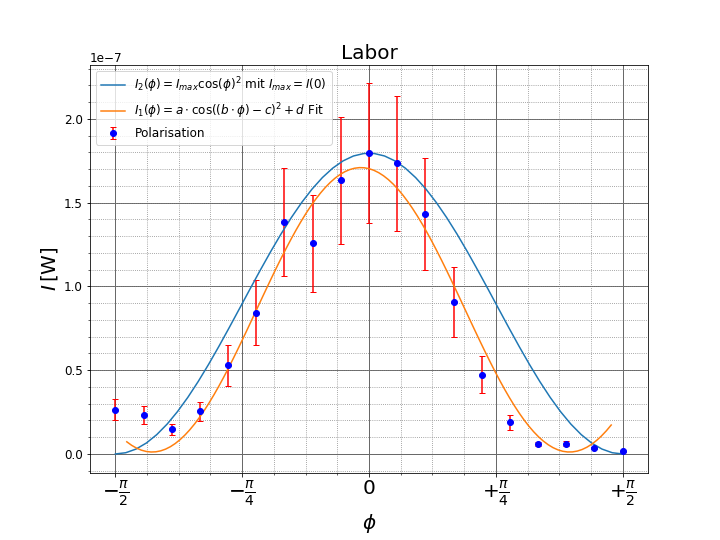
\includegraphics[scale=0.55]{Bilder/Polarisation-Labor}
	\caption{Gemessene Intensität in Abhängigkeit vom Winkel $\phi$ des Empfängers im Großen Hörsaal der Physik. Fehler in $y$-Richtung sind mittels Formel \eqref{deltaI} berechnet und eingetragen. Auch wurde die Funktion $I_{1}(\phi)$ \eqref{I1}  mittels \texttt{curvefit}. (Python Modul \cite{curvescipy}) an die Messwerte geplottet. Auch wurde der theoretische Verlauf nach Formel \eqref{I2} eingetragen.}
	\label{GrH-P}
\end{figure}

\begin{figure}[ht]
	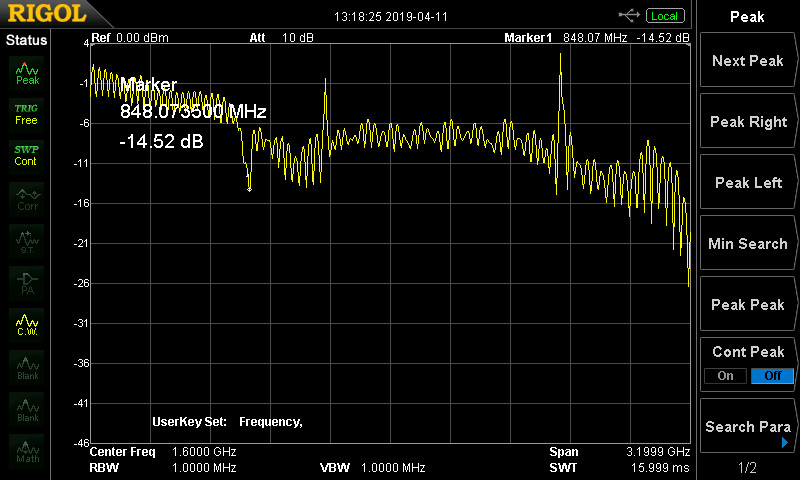
\includegraphics[scale=0.075]{Bilder/ant32.jpg}
	\centering
	\caption{Charakteristik der ersten Antenne, erste Generation. Charakteristische Frequenz $f=848{,}07\,$MHz}
	\label{Ant1alt}
\end{figure}

\begin{figure}[ht]
	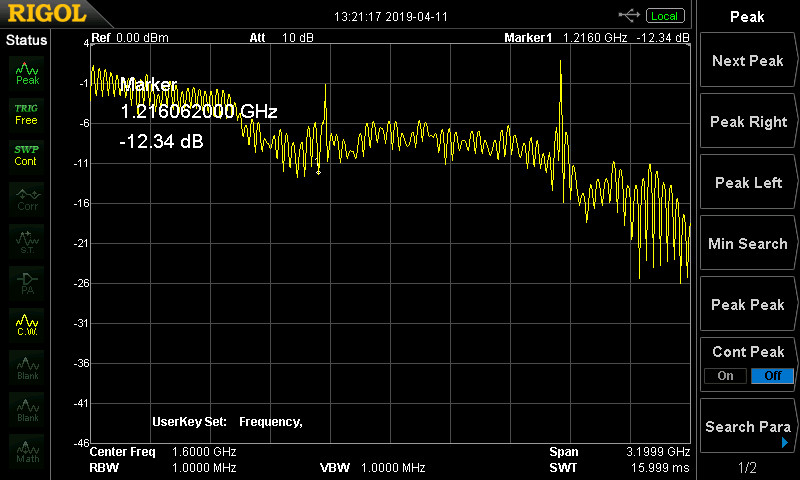
\includegraphics[scale=0.075]{Bilder/ant42.jpg}
	\centering
	\caption{Charakteristik der zweiten Antenne, erste Generation. Charakteristische Frequenz $f=1{,}23\,$GHz}
	\label{Ant2alt}
\end{figure}

\begin{figure}[ht]
	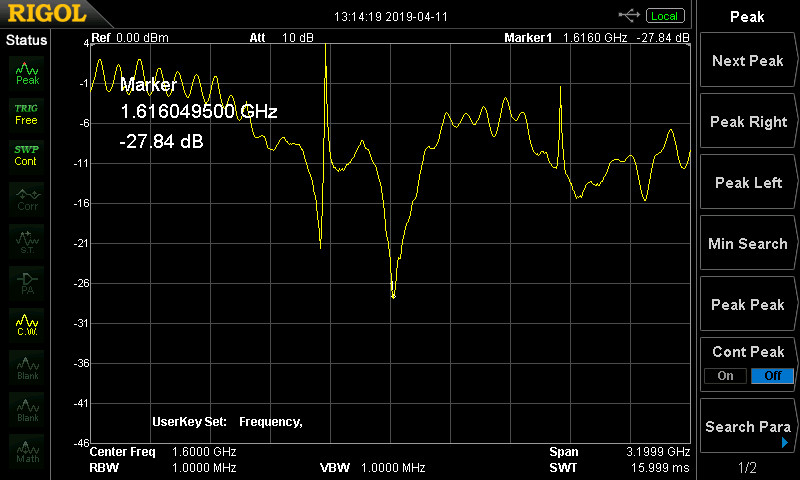
\includegraphics[scale=0.075]{Bilder/ant12.jpg}
	\centering
	\caption{}
	\label{Ant1}
\end{figure}

\begin{figure}[ht]
	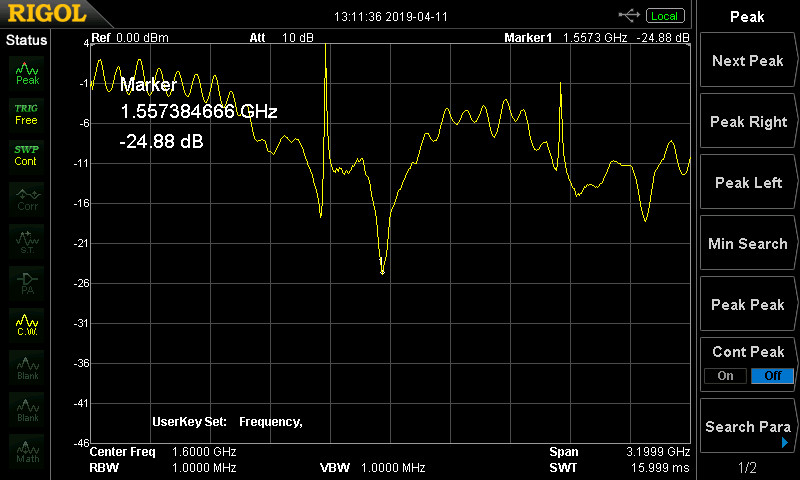
\includegraphics[scale=0.075]{Bilder/ant22.jpg}
	\centering
	\caption{\textcolor{red}{caption Fehlt!!!}}
	\label{Ant2}
\end{figure}

%\begin{figure}[ht]
%	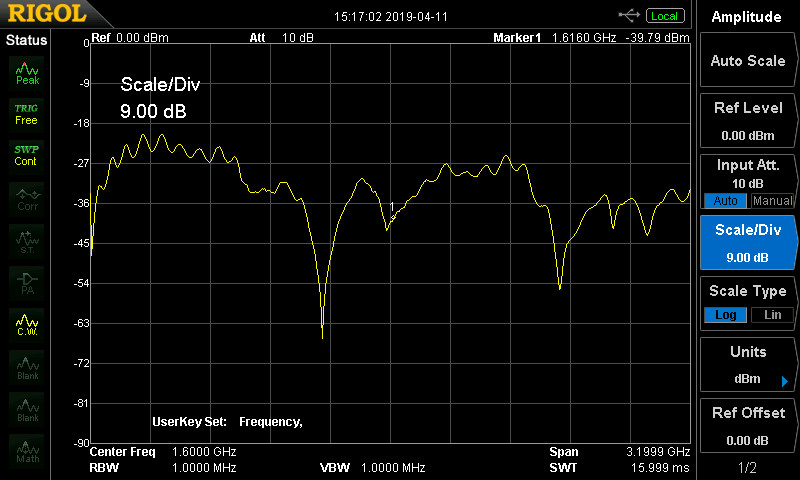
\includegraphics[scale=0.075]{Bilder/anttrimm.jpg}
%	\centering
%	\caption{\textcolor{red}{caption Fehlt!!!} glaube das ist Antenne 2 getrimmt aber ohne Korrektur des Rückkopplers}
%	\label{Ant2-mitrückkoppler}
%\end{figure}

\begin{figure}[ht]
	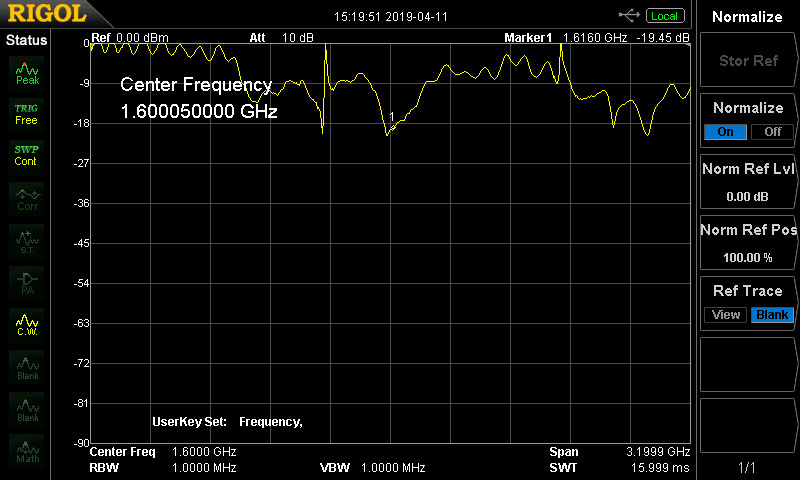
\includegraphics[scale=0.075]{Bilder/anttrimm2.jpg}
	\centering
	\caption{\textcolor{red}{caption Fehlt!!!} das hier Antenne 2 getrimmt und korrigiert}
	\label{Ant2-getrimmt}
\end{figure}

\begin{figure}[ht]
	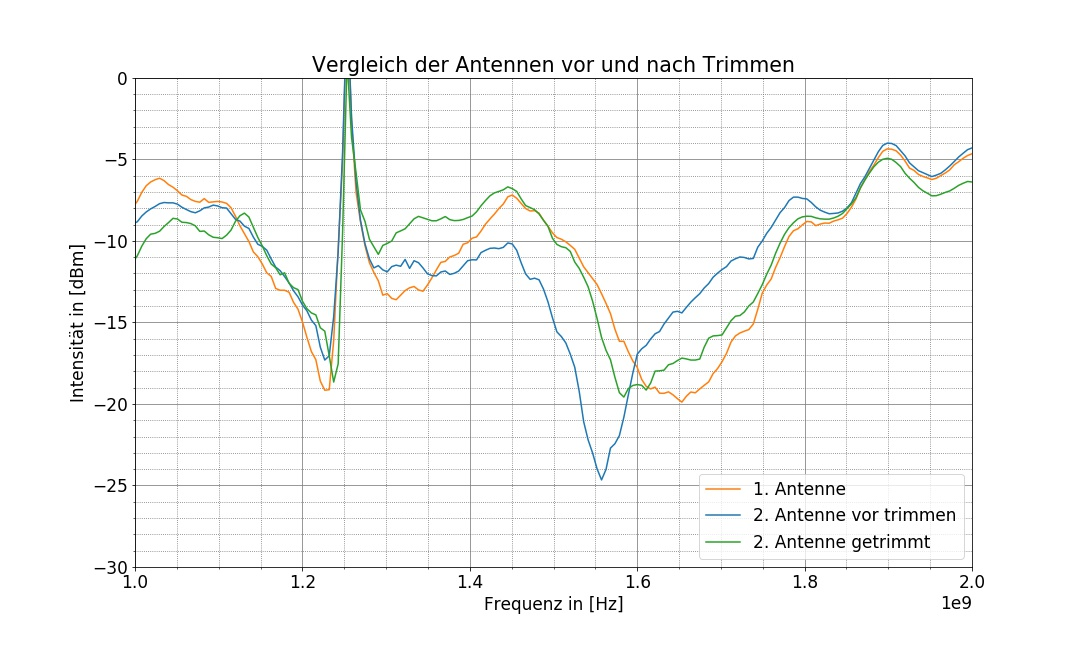
\includegraphics[scale=0.4]{Bilder/Antennentrimmen}
	\centering
	\caption{\textcolor{red}{caption Fehlt!!!} also quasi Abbildunen \ref{Ant1}, \ref{Ant2} und \ref{Ant2-getrimmt}}
	\label{Vergleich}
\end{figure}

\end{document}